\documentclass{article}
\usepackage[margin=1in]{geometry}
\usepackage{amsmath,amsthm,amssymb}
\usepackage{bbm,enumerate,mathtools}
\usepackage{tikz,pgfplots}
\usepackage{chessboard}
\usepackage[hidelinks]{hyperref}
\usepackage{multicol} % Problem 35

\newenvironment{question}{\begin{trivlist}\item[\textbf{Question.}]}{\end{trivlist}}
\newenvironment{note}{\begin{trivlist}\item[\textbf{Note.}]}{\end{trivlist}}
\newenvironment{references}{\begin{trivlist}\item[\textbf{References.}]}{\end{trivlist}}
\newenvironment{related}{\begin{trivlist}\item[\textbf{Related.}]\end{trivlist}\begin{enumerate}}{\end{enumerate}}


\begin{document}

\rating{3}{4}
In a letter, Alec Jones asks notes that there are eleven distinct nets of the
cube, considered as free polyominoes.
\begin{figure}[ht!]
  \centering
  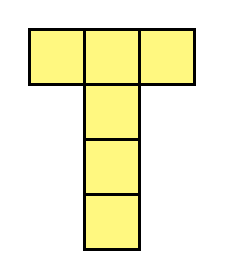
\begin{tikzpicture}[scale=0.7]
    \draw[very thick, line cap=rect, fill=yellow!50] (0,0) grid (3,1) rectangle (0,0);
    \draw[very thick, line cap=rect, fill=yellow!50] (1,0) grid (2,-3) rectangle (1,0);
  \end{tikzpicture}
  ~~~
  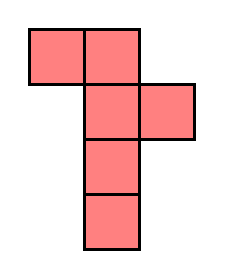
\begin{tikzpicture}[scale=0.7]
    \draw[very thick, line cap=rect, fill=red!50] (0,0) grid (2,1) rectangle (0,0);
    \draw[very thick, line cap=rect, fill=red!50] (1,0) grid (2,-3) rectangle (1,0);
    \draw[very thick, line cap=rect, fill=red!50] (2,0) grid (3,-1) rectangle (2,0);
  \end{tikzpicture}
  ~~~
  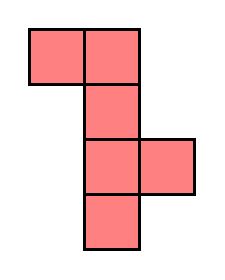
\begin{tikzpicture}[scale=0.7]
    \draw[very thick, line cap=rect, fill=red!50] (0,0) grid (2,1) rectangle (0,0);
    \draw[very thick, line cap=rect, fill=red!50] (1,0) grid (2,-3) rectangle (1,0);
    \draw[very thick, line cap=rect, fill=red!50] (2,-1) grid (3,-2) rectangle (2,-1);
  \end{tikzpicture}
  ~~~
  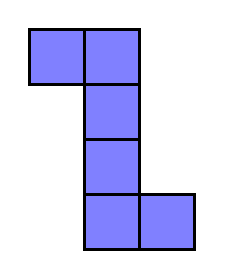
\begin{tikzpicture}[scale=0.7]
    \draw[very thick, line cap=rect, fill=blue!50] (0,0) grid (2,1) rectangle (0,0);
    \draw[very thick, line cap=rect, fill=blue!50] (1,0) grid (2,-3) rectangle (1,0);
    \draw[very thick, line cap=rect, fill=blue!50] (2,-2) grid (3,-3) rectangle (2,-2);
  \end{tikzpicture}
  ~~~
  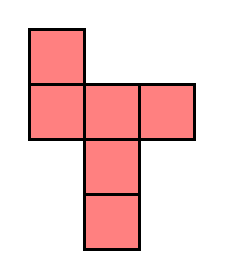
\begin{tikzpicture}[scale=0.7]
    \draw[very thick, line cap=rect, fill=red!50] (0,0) grid (1,-2) rectangle (0,0);
    \draw[very thick, line cap=rect, fill=red!50] (1,-1) grid (2,-4) rectangle (1,-1);
    \draw[very thick, line cap=rect, fill=red!50] (2,-1) grid (3,-2) rectangle (2,-1);
  \end{tikzpicture}
  \\
  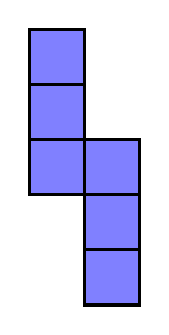
\begin{tikzpicture}[scale=0.7]
    \draw[very thick, line cap=rect, fill=blue!50] (0,0) grid (1,-3) rectangle (0,0);
    \draw[very thick, line cap=rect, fill=blue!50] (1,-2) grid (2,-5) rectangle (1,-2);
  \end{tikzpicture}
  ~~~
  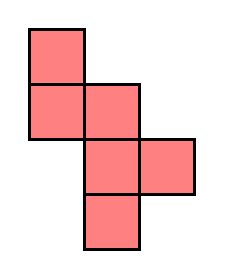
\begin{tikzpicture}[scale=0.7]
    \draw[very thick, line cap=rect, fill=red!50] (0,0) grid (1,-2) rectangle (0,0);
    \draw[very thick, line cap=rect, fill=red!50] (1,-1) grid (2,-4) rectangle (1,-1);
    \draw[very thick, line cap=rect, fill=red!50] (2,-2) grid (3,-3) rectangle (2,-2);
  \end{tikzpicture}
  ~~~
  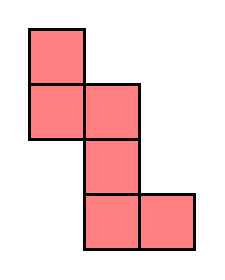
\begin{tikzpicture}[scale=0.7]
    \draw[very thick, line cap=rect, fill=red!50] (0,0) grid (1,-2) rectangle (0,0);
    \draw[very thick, line cap=rect, fill=red!50] (1,-1) grid (2,-4) rectangle (1,-1);
    \draw[very thick, line cap=rect, fill=red!50] (2,-3) grid (3,-4) rectangle (2,-3);
  \end{tikzpicture}
  ~~~
  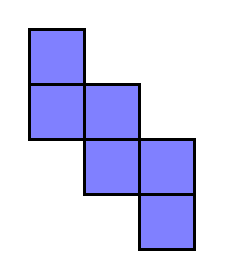
\begin{tikzpicture}[scale=0.7]
    \draw[very thick, line cap=rect, fill=blue!50] (0,0) grid (1,-2) rectangle (0,0);
    \draw[very thick, line cap=rect, fill=blue!50] (1,-1) grid (2,-3) rectangle (1,-1);
    \draw[very thick, line cap=rect, fill=blue!50] (2,-2) grid (3,-4) rectangle (2,-2);
  \end{tikzpicture}
  ~~~
  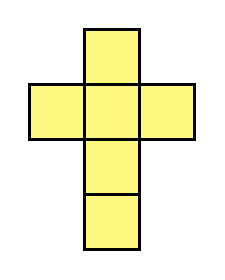
\begin{tikzpicture}[scale=0.7]
    \draw[very thick, line cap=rect, fill=yellow!50] (0,-1) grid (1,-2) rectangle (0,-1);
    \draw[very thick, line cap=rect, fill=yellow!50] (1,0) grid (2,-4) rectangle (1,0);
    \draw[very thick, line cap=rect, fill=yellow!50] (2,-1) grid (3,-2) rectangle (2,-1);
  \end{tikzpicture}
  ~~~
  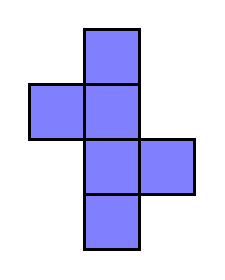
\begin{tikzpicture}[scale=0.7]
    \draw[very thick, line cap=rect, fill=blue!50] (0,-1) grid (1,-2) rectangle (0,-1);
    \draw[very thick, line cap=rect, fill=blue!50] (1,0) grid (2,-4) rectangle (1,0);
    \draw[very thick, line cap=rect, fill=blue!50] (2,-2) grid (3,-3) rectangle (2,-2);
  \end{tikzpicture}
  \caption{
    Eleven distinct nets of the ($3$-hyper)cube.
    Two, marked in yellow, have reflection symmetry, that is they are achiral;
    four, marked in blue, have rotational symmetry.
  }
\end{figure}

\begin{question}
  Alec asks, how many nets are there of the $n$-hypercube?
\end{question}

\begin{related}
  \item How many of the nets exhibit some sort of symmetry, as shown in the example.
  \item How many nets are there of the $n$-simplex? Other polyhedra?
  \item How many nets for a rectangular analog? That is for some $a_1, a_2, \hdots, a_n$, \[
    R = \{(x_1, x_2, \hdots, x_n) : x_i = 0 \text{ or } x_i = a_i\}.
  \] Note that in the case of the $n$-hypercube, $a_1 = a_2 = \hdots = a_n = 1$.
  \item Must all of these nets ``use up'' $n$ dimensions.
  (In the case of $n=3$ in the example, yes, because the ``straight line''
  $6$-omino cannot be folded into a cube.)
  \item What is the net with the smallest convex hull by hypervolume? Largest?
  \item How many of the nets tile $(n-1)$-space?
\end{related}

\begin{note}
  There is $1$ net for the $2$-hypercube, $11$ nets for the $3$-hypercube,
  and $261$ nets for the $4$-hypercube.
  The answer is unknown for the $5$-hypercube.
  The corresponding sequence is tagged ``hard'' on OEIS.
\end{note}

\begin{references}
  \item \url{https://oeis.org/A091159}
  \item \url{https://mathoverflow.net/q/198722/104733}
\end{references}

\end{document}
